\PassOptionsToPackage{unicode=true}{hyperref} % options for packages loaded elsewhere
\PassOptionsToPackage{hyphens}{url}
%
\documentclass[]{article}
\usepackage{lmodern}
\usepackage{amssymb,amsmath}
\usepackage{ifxetex,ifluatex}
\usepackage{fixltx2e} % provides \textsubscript
\ifnum 0\ifxetex 1\fi\ifluatex 1\fi=0 % if pdftex
  \usepackage[T1]{fontenc}
  \usepackage[utf8]{inputenc}
  \usepackage{textcomp} % provides euro and other symbols
\else % if luatex or xelatex
  \usepackage{unicode-math}
  \defaultfontfeatures{Ligatures=TeX,Scale=MatchLowercase}
\fi
% use upquote if available, for straight quotes in verbatim environments
\IfFileExists{upquote.sty}{\usepackage{upquote}}{}
% use microtype if available
\IfFileExists{microtype.sty}{%
\usepackage[]{microtype}
\UseMicrotypeSet[protrusion]{basicmath} % disable protrusion for tt fonts
}{}
\IfFileExists{parskip.sty}{%
\usepackage{parskip}
}{% else
\setlength{\parindent}{0pt}
\setlength{\parskip}{6pt plus 2pt minus 1pt}
}
\usepackage{hyperref}
\hypersetup{
            pdfborder={0 0 0},
            breaklinks=true}
\urlstyle{same}  % don't use monospace font for urls
\usepackage[margin=1.0in]{geometry}
\usepackage{graphicx,grffile}
\makeatletter
\def\maxwidth{\ifdim\Gin@nat@width>\linewidth\linewidth\else\Gin@nat@width\fi}
\def\maxheight{\ifdim\Gin@nat@height>\textheight\textheight\else\Gin@nat@height\fi}
\makeatother
% Scale images if necessary, so that they will not overflow the page
% margins by default, and it is still possible to overwrite the defaults
% using explicit options in \includegraphics[width, height, ...]{}
\setkeys{Gin}{width=\maxwidth,height=\maxheight,keepaspectratio}
\setlength{\emergencystretch}{3em}  % prevent overfull lines
\providecommand{\tightlist}{%
  \setlength{\itemsep}{0pt}\setlength{\parskip}{0pt}}
\setcounter{secnumdepth}{0}
% Redefines (sub)paragraphs to behave more like sections
\ifx\paragraph\undefined\else
\let\oldparagraph\paragraph
\renewcommand{\paragraph}[1]{\oldparagraph{#1}\mbox{}}
\fi
\ifx\subparagraph\undefined\else
\let\oldsubparagraph\subparagraph
\renewcommand{\subparagraph}[1]{\oldsubparagraph{#1}\mbox{}}
\fi

% set default figure placement to htbp
\makeatletter
\def\fps@figure{htbp}
\makeatother

\usepackage{palatino}
\usepackage{setspace}
\doublespacing
\usepackage[left]{lineno}
\linenumbers

\author{}
\date{\vspace{-2.5em}}

\begin{document}

\hypertarget{environmental-and-genetic-contributions-to-ecogeographic-rules-in-house-mice}{%
\section{Environmental and genetic contributions to ecogeographic rules
in house
mice}\label{environmental-and-genetic-contributions-to-ecogeographic-rules-in-house-mice}}

\vspace{20mm}

Mallory A. Ballinger and Michael W. Nachman\({^\dagger}\)

\vspace{20mm}

Department of Integrative Biology

Museum of Vertebrate Zoology

University of California, Berkeley

Berkeley, CA 94702-3160

\vspace{10mm}

\({\dagger}\) To whom orrespondence should be addressed:

\href{mailto:mnachman@berkeley.edu}{mnachman@berkeley.edu}

\vspace{40mm}

\textbf{Running title:} Allen's rule and Bergmann's rule in house mice

\newpage

\hypertarget{abstract-200-words}{%
\subsection{Abstract (200 words)}\label{abstract-200-words}}

Distinguishing between genetic, environmental, and
genotype-by-environment effects are central to understanding geographic
variation in phenotypic clines. Two of the best-documented phenotypic
clines are Bergmann's rule and Allen's rule, which predict larger body
sizes and shortened extremities in colder climates, respectively.
Although numerous studies have found evidence for both ecogeographic
patterns within and across taxa, we still have little understanding
about whether these patterns are driven by genetics, environment, or
both. Here, we measure the genetic and environmental contributions of
Bergmann's rule and Allen's rule across introduced populations of
American house mice (\emph{Mus musculus domesticus}). First, we document
patterns of Bergmann's rule and Allen's rule in wild-caught house mice
across North and South America, with larger body sizes and shortened
extremities present at higher latitudes. Next, we find genetically based
differences in body mass and tail length between mice from upstate New
York and equatorial Brazil, patterns consistent with Bermgann's rule and
Allen's rule. We then assess the contributions of phenotypic plasticity
to these ecogeographic patterns and found very little plasticity in body
size across both populations. Unlike body size, we found considerable
plasticity in extremity length in response to cold temperature. The
plastic responses of tail length and ear length goes in the same
direction as the evolved responses, highlighting an example of adpative
phenotypic plasticity underlying Allen's rule.

\newpage

\hypertarget{introduction}{%
\subsection{Introduction}\label{introduction}}

Clines in phentoypes have historically been attributed to natural
selection and reflect adaptation to local environments (Huxley 1938;
Endler 1977). Two of the most well described phenotypic clines are
Allen's rule and Bergmann's rule. Allen's rule predicts that extremities
of organisms occupying cold geographic regions are shorter compared to
conspecifics occupying warm regions (Allen 1877). Similarly, Bergmann's
rule predicts larger body sizes in colder climates compared to organisms
occupying warmer climates (Bergmann 1847). Shortened extremities and
larger body sizes minimize heat loss by reducing surface area to volume
ratios and are viewed as thermoregulatory adaptations (Mayr 1956).
Numerous studies have documented Bergmann's rule and Allen's rule within
and across species of birds (Snow 1954; James 1970; Johnston and
Selander 1971) and mammals (Brown and Lee 1969; Griffing 1974; Yom-Tov
and Nix 1986), including humans (Ruff 1994; Foster and Collard 2013;
Betti et al. 2015). Moreover, various meta-analyses have supported
({\textbf{???}}; {\textbf{???}}; Freckleton et al. 2003; Meiri and Dayan
2003; Blackburn and Hawkins 2004; Millien2006; Olson2009; Symonds and
Tattersall 2010; Nudds and Oswald 2007; Alhajeri et al. 2020) or refuted
({\textbf{???}}; {\textbf{???}}; McNab 1971; Geist 1987) an evolutionary
basis to these phenotypic clines. The contradicting results found across
the literature are unsurprising given the variation within and among
datasets, such as choice of taxonomic groups, environmental variables,
and inconsitencies in morphological measurements. To date, we still have
very little understanding of the mechanisms underlying Allen's rule and
Bergmann's rule.

Missing from many of these discussions are careful analyses determining
which traits are genetically encoded, environmentally influenced, or
both. Most traits associated with Bergmann's rule and Allen's rule are
quantitative, meaning they are polygenic and environmentally determined
{[}Lynch and Walsh 1998; Falconer and Mackay 1996{]}. Disentangling
genetics from environmental effects in natural populations is difficult
when solely using phenotypic data collected from wild-caught specimens.
Patterns consistent with Bergmann's rule and Allen's rule may exist
underneath environmental effects and possible genotype-by-environment
ineratctions ({\textbf{???}}; Conover and Schultz 1995). Phenotypic
plasticity may also generate clinal patterns, giving a false indication
for adaptive clines ({\textbf{???}}; James 1983). In fact, many temporal
patterns of Bergmann's rule are driven by the environment
(i.e.~nonadaptive plasticity) and not genetic adaptation in birds
(Teplitsky et al. 2008; Husby et al. 2011) and mammals (Ozgul et al.
2009, 2010). Furthermore, we have little understanding how populations
conforming to these ecogeographic rules vary in the degree or direction
of plasticity they exhibit in response to environmental stimuli.
Variation in plasticity and gentoype-by-environment interactions may
faciliate adaptation and divergence in polygenic traits such as body
size (Via and Lande 1985; Gillespie and Turelli 1989; Gomulkiewicz and
Kirkpatrick 1992). However, controlling for environmental effects and
measuring the contributions of phenotypic plasticity is difficult, as
transplant experiments and common garden experiments are infeasible for
many taxa. These limitations have impeded our ability to make
substantial progress on understanding the evolutionary and ecological
mechanisms underlying Bergmann's rule and Allen's rule.

House mice (\emph{Mus musculus domesticus}) are a tractable system to
dissentangle genetics from environment underlying complex traits. House
mice have recently expanded their range from Western Europe to the
Americas, where they can be found from the tip of South America up to
Alaska. Across this broad latitudinal range, house mice are exposed to
considerable variation in climatic conditions, including cold, temperate
environments to warm, tropical and arid environments ({\textbf{???}}).
Despite house mice residing in these novel environments for only
\textasciitilde{}500 generations, there is evidence for clinal
adaptation across populations. Specifically, mice in eastern North
America follow Bergmann's rule (Lynch 1992), with larger mice in more
northern populations compared to their southern conspecifics. These body
size differences persist in a commmon environment and over many
generations, indicating a genetic basis for Bergmann's rule in house
mice ({\textbf{???}}; Lynch 1992). Experimental evolution studies of
house mice conducted in the laboratory recapitulate these clinal
patterns, in which mice evolved at lower temperatures become larger and
undergo genetic divergence in body size (Barnett and Dickson 1984).
Furthermore, earlier work revealed an environmental influence on tail
length when exposed to cold temperatures. Specficially, house mice
reared in a cold environment grew significantly shorter tails than mice
reared at warm temperatures, consistent with Allen's rule
({\textbf{???}}; {\textbf{???}}; Barnett 1965). However, these earlier
studies either only investigated a single population of wild house mice
or used traditional laboratory strains of mice, making it difficult to
place the results in an explicit evolutionary framework. We still have
little understanding of the phenotpic variation of house mice across
their entire latitudinal distribution, and the subsequent contributions
of genetics and the enviornment on these complex traits.

Here, we use a combination of approaches to tease apart genetics from
plasticity in Bergmann's rule and Allen's rule in American house mice.
First, we determined if house mice conform to both Bergmann's rule and
Allen's rule across their entire introduced range by analyzing
phenotypic data from wild-caught individuals across North and South
America. Second, because it is difficult to dissentangle genetics from
plasticity using wild phenotypic data, we collected temperate and
tropical populations of house mice from the ends of their latitudinal
distribution, brought them back to the lab, and established wild-derived
colonies. We analyzed phenotypic differences between populations and
across generations in a common environment to identify a genetic basis
for Allen's rule and Bergmann's rule. Third, to measure the influence of
environment on body size and extremity length, we performed a second
common garden experiment by rearing both populations of house mice in a
cold environment and measured the effects on body size and extremity
length. Measuring developmental plasticity in these traits allows us to
assess the influence of temperature on Bergmann's rule and Allen's rule.
Specifically, we show that unlike body size, extremity length is highly
plastic, and this plastic response goes in the same direction as the
evolved response, highlighting an example of adaptive phentoypic
plasticity.

\newpage

\hypertarget{materials-and-methods}{%
\subsection{Materials and Methods}\label{materials-and-methods}}

\hypertarget{wild-caught-phenotypic-metadata}{%
\subparagraph{\texorpdfstring{\emph{Wild-caught phenotypic
metadata}}{Wild-caught phenotypic metadata}}\label{wild-caught-phenotypic-metadata}}

To determine if house mice conform to Allen's rule and Bergmann's rule,
we assessed the relationship between body mass, tail length, ear length,
and latitude in wild house mice collected across North and South
America. Specimen data of all house mouse records were downloaded from
VertNet (a Database of Vertebrate Specimen Records)
(\url{http://vertnet.org})(Constable et al. 2010) on October 13, 2020,
using the search query: \emph{vntype}:specimen, \emph{genus}:Mus. We
obtained 62,139 museum records and retained records that included
\emph{Mus musculus} specimens collected in North or South America
(excluding islands). We further excluded individuals listed as pregnant,
juvenile, subadult, or immature, and kept those identified as adult,
mature, or with no age class noted. We also manually coded females and
males as `adult' if they fulfilled any of the following criteria:
females - presence of placental scars, parous, or lactating; males -
presence of seminal vesicles, testes descended (TD), or testes scrotal
(TS). Tail lengths shorter than 20mm and longer than 120mm (\emph{n} =
8), and ear lengths greater than 30mm (\emph{n} = 1) were considered
extreme outliers (greater than 3.5 standard deviations from the mean)
and were removed from downstream analyses, as these likely represent
juveniles or measuring erros. Sample information for the final VertNet
dataset (n = 3,018) is provided in Data S1.

\hypertarget{laboratory-reared-mice---common-garden-experiment-1}{%
\subparagraph{\texorpdfstring{\emph{Laboratory-reared mice - common
garden experiment
1}}{Laboratory-reared mice - common garden experiment 1}}\label{laboratory-reared-mice---common-garden-experiment-1}}

For the first common garden experiment, live animals were collected from
two locations that represent the ends of the latitudinal transect:
Manaus, Amazonas, Brazil (MAN) and Saratoga Springs, New York, USA
(SAR). Details of this common garden experiment are specified in
({\textbf{???}}; Suzuki et al. 2020). Briefly, live mice from both
Brazil and New York were brought back to the lab at the University of
California, Berkeley. Within each population, unrelated pairs of
wild-caught mice were mated to produce first generation (N1) lab-reared
mice, and these inbred lines have subsequently been maintained through
sib-sib matings each generation for over 10 generations. Wild-caught
mice and their descendants were housed in a standard laboratory
environment at 21\textsuperscript{o}C with a 12-hr dark and 12-hr light
cycle. Commerical rodent chow was provided ad libitium. Standard museum
measurements were taken for all wild-caught, N1, and N2 mice from each
population (see Data S3). Tail lengths less than 50mm (\emph{n} = 2) and
ear lengths less than 8mm (\emph{n} = 1) were considered outliers
(greater than three standard deviations away from the mean) and were
removed from downstream analyses.

\hypertarget{developmental-phenotypic-plasticity---common-garden-experiment-2}{%
\subparagraph{\texorpdfstring{\emph{Developmental phenotypic plasticity
- common garden experiment
2}}{Developmental phenotypic plasticity - common garden experiment 2}}\label{developmental-phenotypic-plasticity---common-garden-experiment-2}}

For the second common garden experiment, we used two wild-derived inbred
lines each from Brazil (MANA, MANB) and New York (SARA, SARB). Each line
was over 10 generations of inbreeding. Equal numbers of males and
females were produced for each within-line comparison (n = 656; see Data
S4). Full sibs were born at room temperature (21\textsuperscript{o}C)
and singly-housed at weaning (\textasciitilde{}21 days old). After a
brief acclimation period, 3.5-week-old mice were randomly assigned into
sized matched groups based on sex-specific body mass, and housed at
either 5\textsuperscript{o}C or remained at 21\textsuperscript{o}C for
the duration of the experiment (\textasciitilde{}50 days total). Initial
body weights and tail lengths were measured, and subsequent weekly body
mass and tail lengths were recorded once a week for each mouse. At the
end of the experiment, mice were sacrificed at 75 ± 3 days of age, and
final body masses and tail lengths were taken, in addition to standard
museum measurements. Two final ear lengths were not included in analyses
due to ear damage. Skulls and skeletons of all mice were deposited in
the Museum of Vertebrate Zoology, University of California, Berkeley.
All experimental procedures were in accordance with the UC Berkeley
Institutional Animal Care and Use Committee (AUP-2017-08-10248).

\hypertarget{data-analysis}{%
\subparagraph{\texorpdfstring{\emph{Data
Analysis}}{Data Analysis}}\label{data-analysis}}

All data analyses and visualizations were completed in R (v. 4.0.3).
Within R, we used the tidyverse (v. 1.3.0)(Wickham et al. 2019),
performance (v. 0.7.1)(Lüdecke et al. 2021), cowplot (v. 1.1.1), here
(v. 1.0.1), and rmarkdown (v. 2.7)(Allaire et al. 2021) packages, along
with R base library. Tail length residuals and ear length residuals were
calculated by regressing absolute length from body mass. Residuals
calculated from body mass consistently performed better (lower Akaike's
information criterion (AIC) values across all datasets than residuals
calculated from body length. We controlled for the effect of body size
on extremity length when testing Allen's rule by including body mass as
an additional predictor in all statistical models (Freckleton 2002)). We
controlled for sex-biased variation in morphological measurements by
including sex as a predictor variable in all models.

We tested for clinal patterns of body mass and extremity length across
latitude in wild-caught house mice using Spearman correlations. For
common garden experiment one, we fitted a linear model using lm\{stats\}
to predict body mass, tail length, and ear length with sex, population,
and generation (formula: (trait) \textasciitilde{} Body Mass + Sex *
Population * Environment). The significance of interactions were tested
were evaluated using using summary\{base\} and analysis of variance
(ANOVA) based on type III (partial) sums of squares, implemented in the
CAR library (v. 3.0.10)(Fox and Weisberg 2019). For common garden
experiment two, we fitted a linear mixed model (estimated using
restricted maximum likelihood) using lmer\{lme4\} (v. 1.1.26)(Bates et
al. 2015) to predict body mass, tail length, and ear length with sex,
population and environment (formula: (trait) \textasciitilde{} Body Mass
+ Sex * Population * Environment). The model included line as a random
effect (formula: \textasciitilde{}1 \textbar{} Line). Results were
evaluated using summary\{lmerTest\} (v. 3.1.3)(Kuznetsova et al. 2017)
and Anova\{car\}. We peformed \emph{post hoc} comparisons on significant
two-way interactions using Tukey's HSD tests or Mann-Whitney \emph{U}
tests. The code to perform analyses for this study are available as a
git-based version control repository on GitHub
(\url{https://github.com/malballinger/Ballinger_allenbergmann_XXXX_2021}).
The analysis can be reproduced using a GNU Make-based workflow with
built-in bash tools (v. 3.2.57(1)-release) and R (v. 4.0.3).

\newpage

\hypertarget{results}{%
\subsection{Results}\label{results}}

\hypertarget{evidence-for-bergmanns-rule-and-allens-rule-in-wild-american-house-mice}{%
\subparagraph{\texorpdfstring{\emph{Evidence for Bergmann's rule and
Allen's rule in wild American house
mice}}{Evidence for Bergmann's rule and Allen's rule in wild American house mice}}\label{evidence-for-bergmanns-rule-and-allens-rule-in-wild-american-house-mice}}

We assessed the relationship between tail length, ear length, body mass,
and latitude in mice collected across North and South America to
determine if populations of house mice conform to Allen's rule and
Bergmann's rule. Using a large dataset downloaded from VertNet (n =
3,018, Data S1), we find weak evidence for Bergmann's rule, as body mass
showed a non-significant, positive correlation with latitude across both
males and females (Figure 1A). In contrast, we found stronger evidence
for Allen's rule in American house mice, with tail length (Figure 1C)
and ear length (Figure 1E) showing a significant, negative correlation
with latitude. These patterns of extremeity length largely hold true
across both sexes (Figure 1C, 1E).

Lack of significant evidence for Bergmann's rule in wild house mice is
likely due to the influence of uncontrolled factors (e.g.~age, diet,
health), environmental effects, or phenotypic plasticity. Although we
minimized the inclusion of records of non-adult specimens by removing
recorded pregnant females, juveniles, and subadults, we still see large
variation across all three traits, likely due to various factors that
were not recorded. To reduce this variation, we filtered the VertNet
dataset to only include adult males (Figure 1; n = 445). We see strong
evidence for both Bergmann's rule (Figure 1B) and Allen's rule (Figure
1D, 1F) across adult, male American house mice, highlighting how
variation and noise encompassed in metadata speaks to the difficulty of
collating museum metadata to infer broad ecogeographic patterns.

\hypertarget{differences-in-body-mass-and-tail-length-persist-in-a-common-environment}{%
\subparagraph{\texorpdfstring{\emph{Differences in body mass and tail
length persist in a common
environment}}{Differences in body mass and tail length persist in a common environment}}\label{differences-in-body-mass-and-tail-length-persist-in-a-common-environment}}

Phenotypic clines observed across wild house mouse populations could
represent genetic differences, phenotypic plasticity, or both. To
dissentagnle genetics from plasticity, we collected live mice from the
ends of the latitudinal transect (Manaus, Amazonas, Brazil and Saratoga
Springs, New York, USA) and brought them into a common laboratory
environment. Population-specific differences in body mass in wild-caught
mice (N0) persisted across the first two generations of
laboratory-reared mice (N1 and N2; Figure 2). Specifically, mice from
New York are larger than mice from Brazil (Kruskal--Wallis,
\emph{F}\(_{1,439}\)=282.54, \emph{P}\textless{}0.001) (Figure 2; Figure
S2), and these differences persisted across and within generations
(Mann-Whitney \emph{U}, P \textless{} 0.001). Sex-specific differences
in body mass were also seen across generations, with males being larger
than females (Kruskal--Wallis, \emph{F}\(_{1,439}\)=50.79,
\emph{P}\textless{}0.001) (Figure 2; Figure S2), and the direction and
magnitude of sexual dimorphism was the same among populations of
American house mice (stats). The maintance of body mass differences in a
common environment and across generations suggests a strong genetic
basis in house mice.

Extremity length (i.e.~tail length and ear length) showed considerable
variation across wild-caught mice (N0) and laboratory-reared mice (N1
and N2; Figure 2A). Despite this variation, Brazil mice have longer
tails than New York mice (ANCOVA, \emph{F}\(_{,419}\)=42.12,
\emph{P}\textless{}0.001) (Figure 2B; Figure S2), and these differences
have persisted across generations in a common environment (Tukey's HSD,
P \textless{} 0.001), suggesting a genetic basis for tail length in
house mice. Ear length showed the most variation, with no strong trends
between populations (Figure 2C; Figure S2). Variation in extremity
length could be due to multiple investigators measuring tail length and
ear length across generations, or it could reflect the inherent plastic
nature of extremity length. For example, although tail length decreases
slightly across generations (Figure 2B), it is difficult to discern if
this is due to phenotypic plasticity or noise being captured in the
metadata. Regardless, extremity length shows greater variation than body
mass, even when measured in a common garden experiment.

\hypertarget{extremity-length-and-not-body-size-is-greatly-influenced-by-temperature}{%
\subparagraph{\texorpdfstring{\emph{Extremity length, and not body size,
is greatly influenced by
temperature}}{Extremity length, and not body size, is greatly influenced by temperature}}\label{extremity-length-and-not-body-size-is-greatly-influenced-by-temperature}}

The results presented above identified phenotypic divergence in body
mass and tail length in house mice, with New York mice having shorter
tails and larger body sizes than mice from Brazil, consistent with
Allen's rule and Bergmann's rule. To determine the influence of
phenotypic plasticity on Bergmann's rule and Allen's rule, we performed
a second common garden experiment by rearing laboratory-born mice from
both populations in a cold environment. We used temperature as the
environmental variable as differences in temperature explain the
majority of phenotypic variation in house mice across North and South
America (Suzuki et al. 2020). Evolved differences in body mass were
evident at weaning (Figure 3), with New York mice larger than Brazil
mice. These body mass differences persisted across development and sex,
and were not influenced by temperature (Figure 3; Figure 5; Figure S3),
and recapitulate patterns seen across generations, with New York mice
larger than Brazil mice (\(\chi^2\)=4, \emph{P}\textless{}0.05), and
males are larger than females (\(\chi^2\)=42.15,
\emph{P}\textless{}0.001). The lack of plasticity in body mass is not a
result of differences in fat accumulation, as body mass index (BMI) does
not differ between populations (\(\chi^2\)=0.50,
\emph{P}\textgreater{}0.05) or environments (\(\chi^2\)=1.28,
\emph{P}\textgreater{}0.05) (Figure S4; Figure S5). This suggests that
phenotypic plasticity plays a modest role in body size evolution of
house mice.

In contrast to body mass, tail length is greatly influenced by
developmental temperature, with the first few weeks post-weaning having
the greatest influence on absolute tail length (Figure 4). Specifically,
mice reared in a cold enviornment grew shorter tails than mice reared in
a warm environment (ANCOVA, \(\chi^2\)=86.05, \emph{P}\textless{}0.001;
Tukey's HSD, \emph{P}\textless{}0.01). Despite developmental temperature
playing a signficant role in tail length, evolved differences in tail
length were evident at the end of the experiment, with Brazil mice
growing longer tails than New York mice (ANCOVA, \(\chi^2\)=11.71,
\emph{P}\textless{}0.001) (Figure 6; Figure S3). Thus, tail length
exhibits both divergence between populations and phenotypic plasticity
between environments. Similarly, cold-reared mice grew shorter ears than
warm-reared mice (ANCOVA, \(\chi^2\)=57.66, P\textless{}0.001) (Figure
6; Figure S3), with no population-specific differences. These
temperature-growth reponses of the extremeites are not a simple
consequence of body size modification, as body size does not differ
between treatments (Figure 5). Overall, unlike body size, extremity
length showed significant plasticity in response to temperature, with
mice growing shorter extremities in a cold environment, consistent with
patterns of Allen's rule.

\hypertarget{adaptive-phenotypic-plasticity-in-extremity-length}{%
\subparagraph{\texorpdfstring{\emph{Adaptive phenotypic plasticity in
extremity
length}}{Adaptive phenotypic plasticity in extremity length}}\label{adaptive-phenotypic-plasticity-in-extremity-length}}

Differences between warm- and cold-reared mice revealed a strong plastic
response to temperature in extremity length. Because plasticity is
considered adaptive when a phenotype is altered in the same direction as
under selection ({\textbf{???}}), we next asked whether phenotypic
plasticity of Brazil mice goes in the same or opposite direction as the
evolved response of New York mice. For tail length, the plastic response
in Brazil house mice recapitulates the evolved tail length of New York
mice (Figure 6A), highlighting an example of adaptive phenotypic
plasticity. Interestingly, the plastic response of New York tail length
is blunted in comparison to Brazil's (Figure 6A), suggesting that New
York house mice are closer to the phenotypic optimum and confer a
greater evolved capacity to cold temperatures. Lastly, plasticity in ear
length of Brazil house mice goes in the same direction as the plastic
response of New York house mice (Figure 6B), again highlighting an
example of adaptive phenotypic plasticity. The overall degree and
directionality of plasticity in extremities mirrors patterns associated
with Allen's rule.

\newpage

\hypertarget{discussion}{%
\subsection{Discussion}\label{discussion}}

We describe phenotypic patterns consisten with Bergmann's rule and
Allen's rule in house mice collected across the Americas. We also
dissentangle the associated contributions of genetics and plasticity to
these ecogeographic patterns. First, we found that wild house mice
conform to Bermgann's rule and Allen's rule, as house mice were smallest
with the longest extremities in the tropics and increased in size with
shortened extremities with increasing latitude. Second, comparisons
between temperate and tropical house mice reared in a common environment
revealed phenotypic differences corresponding to Bergmann's rule and
Allen's rule. Because differences in body mass and tail length persisted
in a common environment across many generations indicates a genetic
basis and represent divergence between the two populations. These
phenotypic differences presumably have arisen as an adpative response to
novel thermal environments. Finally, we measured the contributions of
phenotypic plasticity underlying these ecogeographic patterns and
revealed that extremity length is highly plastic in response to cold
temperature, while body size is unaffected. This plastic response in
extremity length seems to be adaptive as it goes in the same direction
as the evolved response seen in temperate house mice.

\hypertarget{genetic-contributions-to-ecogeographic-rules}{%
\subparagraph{\texorpdfstring{\emph{Genetic contributions to
ecogeographic
rules}}{Genetic contributions to ecogeographic rules}}\label{genetic-contributions-to-ecogeographic-rules}}

Parallel phenotypic clines across multiple transects provide strong
evidence for natural selection (Endler 1977). Body mass in house mice
increases as latitude increases (Figure 1A-B), resembling patterns seen
in eastern North America (Lynch 1992; Phifer-Rixey et al. 2018), South
America (Suzuki et al. 2020), and Australia (Tomlinson and Withers
2009). These clinal patterns are consistent with Bergmann's rule and
reflect an evolved response to differences in environmental temperature.
Phenotypic measurements of second- and tenth-generation lab-reared mice
from temperate and tropical populations demonstrated a genetically
determined difference in body mass (Figure 2A). These results agree with
previous studies also finding a genetic basis for Bergmann's rule in
house mice from eastern North America (Lynch 1992; Phifer-Rixey et al.
2018), western North America (Ferris et al. 2021), and South America
(Suzuki et al. 2020), and suggests that there has been strong selection
for body size in house mice. The strong selection over short time scales
for Bergmann's rule has also been shown for other non-native species,
such as \emph{Drosophila}, which is one of the best-documented examples
for a genetic basis of Bergmann's rule. Specifically, body size clines
in \emph{Drosophila} have been repeated across continents (refs), in
common garden experiments (refs), and through experimental evolution
studies (Anderson 1966, 1973; Cavicchi et al.~1985; Partridge et
al.~1994a,b). The formation of Bergmann's rule has also occurred rapidly
across introduced populations of house sparrows {[}({\textbf{???}});
Packard1967; Baker1980; Fleischer and Johnston 1982; Murphy1885{]} and
starlings ({\textbf{???}}). These results suggest that introduced
species may experience strong selection as they rapidly expand their
geographic range into new environments, and thus clines such as
Bergmann's rule are able to establish rapidly.

Patterns for Allen's rule were consistent for tail length only, with
mice from the equator having longer tails than mice from higher
latitudes (Figure 1C-D). These patterns are recapitualed in the lab and
across generations, demonstrating a genetic basis for tail length
(Figure 2B). Shorter tails in northern populations of house mice likely
confers selection for heat conservation and adaptation to the cold, as
tail length shows a positive correlation with tempeature of the coldest
month across rodents (Alhajeri et al. 2020). Similar trends and
correlations have also been found for appendage length and bill length
in birds (REFs). Alternative mechanisms for Allen's rule have been
postulated to explain why longer tails are found in the tropics, such as
increased climbing ability associated arboreal environments
({\textbf{???}}; Mincer and Russo 2020). Because house mice are
commensal with humans, it is unlikely that longer tails confer a
climbing advantage in the tropics, though this warrants future
investigation. Furthermore, unlike tail length, we do not see a genetic
basis for ear length in American hosue mice (Figure 2C). Although ear
length shows a negative correlation with latitude (Figure 1E-F), this is
likely driven by geographic variation in precipitation rather than
temperature (Alhajeri et al. 2020). Again, this result highlights
alternative mechanisms of Allen's rule, such as primary productivity,
and not just thermoregulation (James 1970; Alhajeri and Steppan 2016).

\hypertarget{contributions-of-phenotypic-plasticity-to-ecogeographic-rules}{%
\subparagraph{\texorpdfstring{\emph{Contributions of phenotypic
plasticity to ecogeographic
rules}}{Contributions of phenotypic plasticity to ecogeographic rules}}\label{contributions-of-phenotypic-plasticity-to-ecogeographic-rules}}

Body size in house mice shows very little plasticity in response to cold
temperature (Figures 3 and 5), reaffirming that there has likely been
strong selection for body size in house mice. Lack of plasticity
associated with Bergmann's rule in house mice is consistent with
previous studies (Sumner refs; Ashoub; Serrat 2008; Serrat 2013) and may
be due to a number of physiological factors. First, the environmental
influence of cold temperature may need to occur pre-weaning or prenatal
to elicit a plastic response, as seen in previous studies of mammals and
birds (refs in serrat paper). Second, temperatures pushing enodtherms
outside their thermoneutral zone have repeatadly been shown to reduce
body mass {[}({\textbf{???}}); ({\textbf{???}});{]}. Although the
plastic response to warm temperatures will likely be different in Brazil
mice compared to New York mice, since Brazil mice are small in body size
and thus likely better at dissipating heat (James1970). Furthermore,
environmental factors other than temperature, such as food availability,
likely elicits a plastic response for body size in house mice (refs),
again highlighting alternative mechanisms undelrying Bergmann's rule
other than temperature (refs). Finally, traits that confer immediate
heat conservation, such as increased fur insulation, may be an intial
plastic response associated with Bergmann's rule and not body size
itself (Scholander 1955).

Unlike Bergmann's rule, Allen's rule can solely be generated via
phenotypic plasticity, as extremity length is highly senstive to ambient
temperature in both mammals and birds (REFs). For example, bill length,
a major thermoregulatory organ of birds (Tattersal 2009), responds
negatively to cold temperatures across populations (refs), presumably as
a strategy for heat conservation. Additionally, numerous studies have
documented the plastic nature of tail length and ear length in
laboratory mice, with both traits responding negatively to cold
temperatures (refs). Our results in wild house mice agree with previous
studies on laboratory mice, with mice growing shorter tails and ears in
a cold environment (Figure 6). This plastic nature of tail length is
also seen at the skeletal level, with both the length and number of
caudal vertebrae decreasing in response to cold temperatures (refs).
Cold temperature direclty effects the growth of cartilage in both tails
and ears, and thus modulates temperature within developing cartilage,
impacting extremity length ({\textbf{???}}). Although we did not measure
skeletal differences among mice, it is likely that the tail length
plasticity we observed is a result of plasticity in both number and
length of individual caudal vertebrae, as seen in other studies of wild
mice (Thorington 1977; Ashboud).

\hypertarget{adaptive-phenotypic-plasticity-and-allens-rule}{%
\subparagraph{\texorpdfstring{\emph{Adaptive phenotypic plasticity and
Allen's
rule}}{Adaptive phenotypic plasticity and Allen's rule}}\label{adaptive-phenotypic-plasticity-and-allens-rule}}

Measuring phenotypic plasticity within and among locally adapted
populations allows us to discern the directionality of plasticity
underlying Allen's rule. Because extremities are strongly influenced by
ambient temperature, plasticity may play an initial role in generating
Allen's rule. Adaptive plasticity is expected to align with the
direction of selection, moving traits closer to the optima (Ghalambor
2007). Our finding that plastic responses of tail length and ear length
in Brazil house mice align with evolved responses of New York house mice
is within the context of adaptive phenotypic plasticity (Ghalamobor
2007; Partridge 1994; Evolution). Specifically, both selection and
plasticity produce shorter tails and ears at lower temperatures. The
plastic response of Brazil tail length matches the evolved response of
New York mice, suggesting that phenotypic plasticity moves mice to the
optimum trait value. Although there has likely been directional
selection in both Brazil mice and New York mice, the plastic responses
observed here are likely similar to the ancestral plastic response,
given the universal response of extremities to temperature in mice
(reviewed in Serrat, 2014).

Furthermore, we expected that New York house mice would have an
attentuted response to the cold environment as they have evolved in a
temperate environment, regularly undergoing seasonal exposure to regular
periods of cold during the winter. In line with this, we observed a
canalized plastic response for tail length in New York house mice,
likely reflecting New York mice being close to the phenotypic optimum.
This canalized response may also be due to skeletal constraint, as the
number and length of caudal vertebrae have been shown to be affected by
temperature (refs). Moreover, genetic assimilation may have likely
played a role in generating shorter tails in colder climates (EXPAND
UPON). Overall, the plastic responses of extremity length mirror evolved
patterns of Allen's rule, and thus may play an important first step in
generating ecogeographic pattern and allowing house mice and other
non-native species are able to expand their geographic range into new
enviornments rapidly.

\newpage

\hypertarget{figures}{%
\subsection{Figures}\label{figures}}

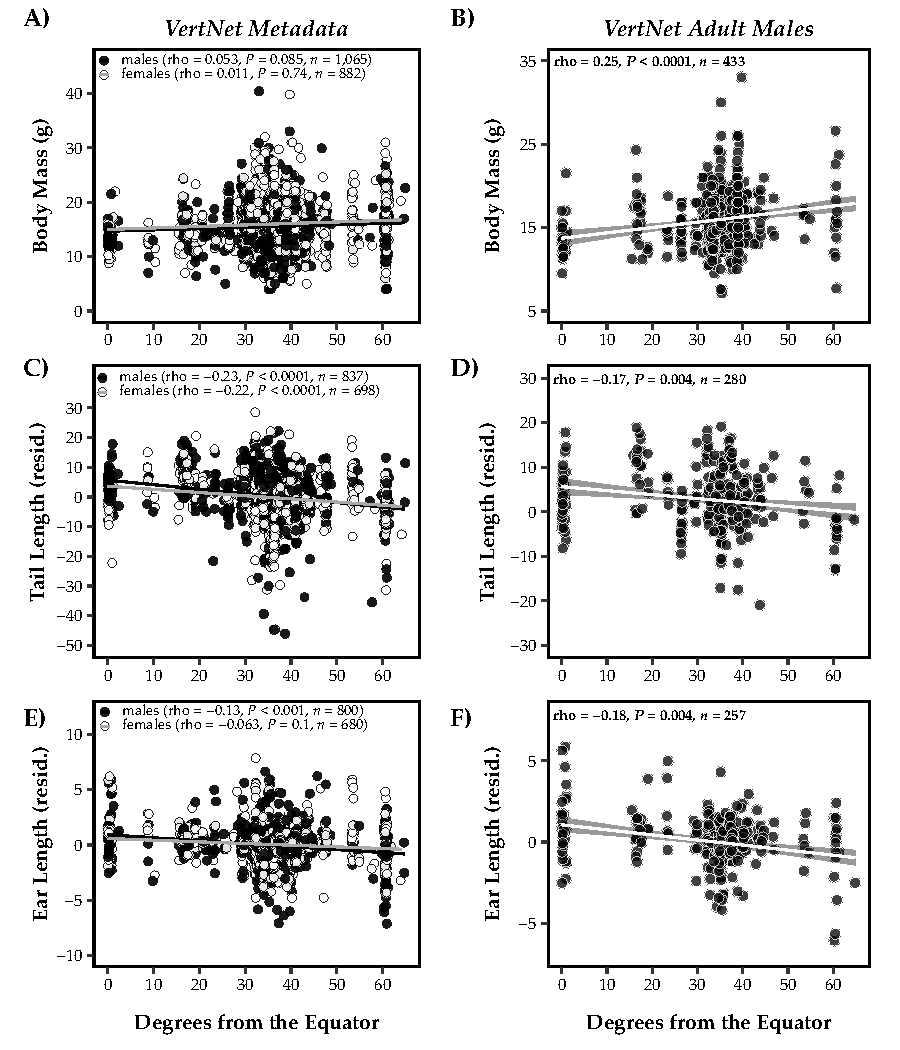
\includegraphics{../results/figures/VertNet_all.pdf}

\textbf{Figure 1. Bergmann's rule and Allen's rule in American house
mice.} The relationship between body mass (A-B), tail length (C-D), ear
length (E-F) and absolute latitude across wild-caught North and South
American house mice. Tail length and ear length are plotted as the
residuals of a regression of body mass on extremity length. Individuals
are represented as individual points, with males denoted as black and
females denoted as white. Results from Spearman correlations are
presented in each plot, along with sample sizes. For clarity, standard
error shading is ommitted from linear regression lines associated with
the VertNet Metadata panels (A,C,E).

\newpage

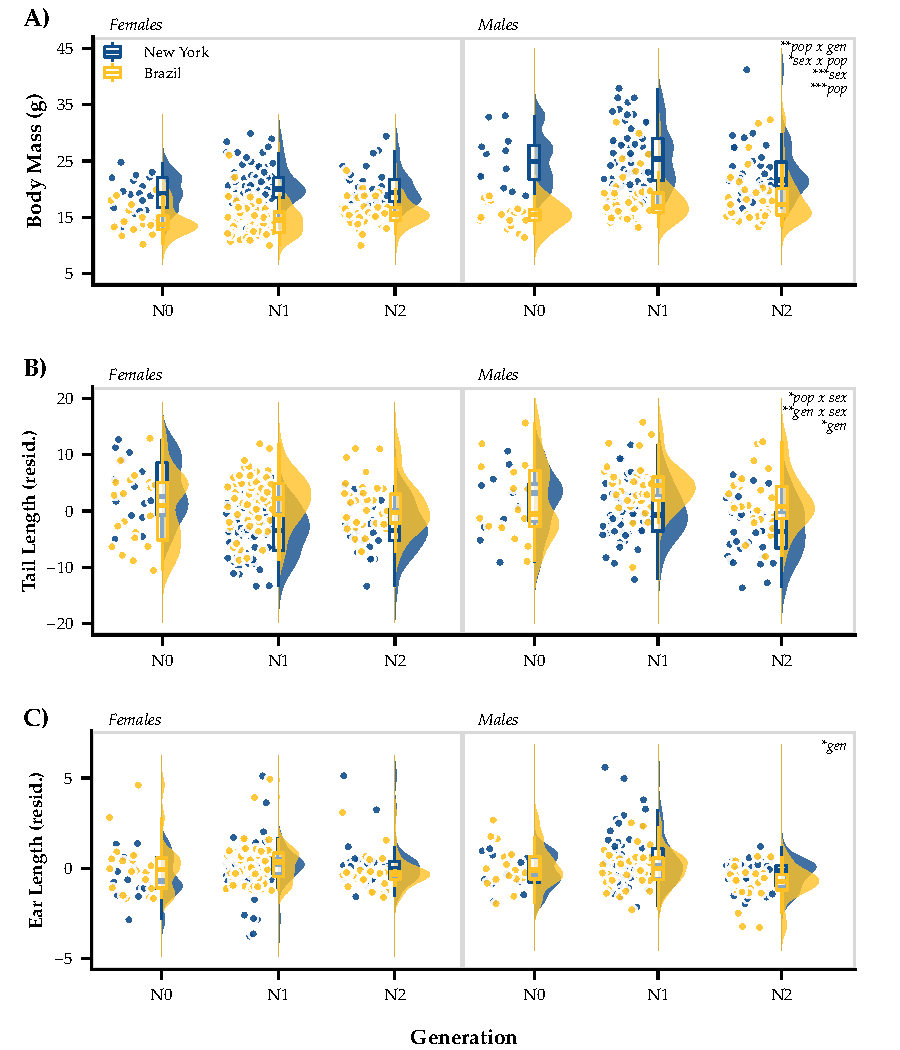
\includegraphics{../results/figures/Generations_colony.pdf}

\textbf{Figure 2. Body mass and tail length differences among
populations persist over generations in a common lab environment.} Tail
length and ear length are plotted as the residuals of a regression of
body mass on extremity length. Population-level data are depticted as
boxplots overlayed on density plots, with boxplot vertical lines
denoting 1.5x the inerquartile range. Individuals are represented as
individual points, and the horizontal variation within each generation
determined randomally to separate points. The New York population is
represented in blue and the Brazil population represented in gold.
Results from linear models are presented in each plot. Sample sizes: (A)
n = 441; (B) n = 432; (C) n = 434.

\newpage

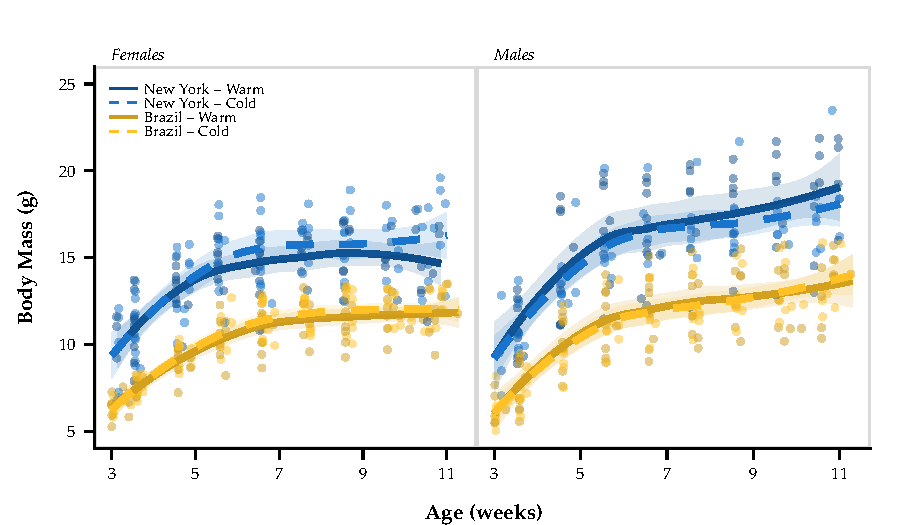
\includegraphics{../results/figures/Weekly_BW.pdf}

\textbf{Figure 3. Evolved differences in body mass across development.}
Body mass growth trajectories across environments in New York (blue) and
Brazil (gold) house mice. Within populations, cold-reared mice (dotted
lines) and warm-reared mice (solid lines) have the same body mass across
development, while males grow larger than females. Individuals are
plotted as semi-transparent points (n = 80), with population means
depicted as smoothed regression fits, with standard error shading. The
same individuals depicted here are also depicted in Figure 5.

\newpage

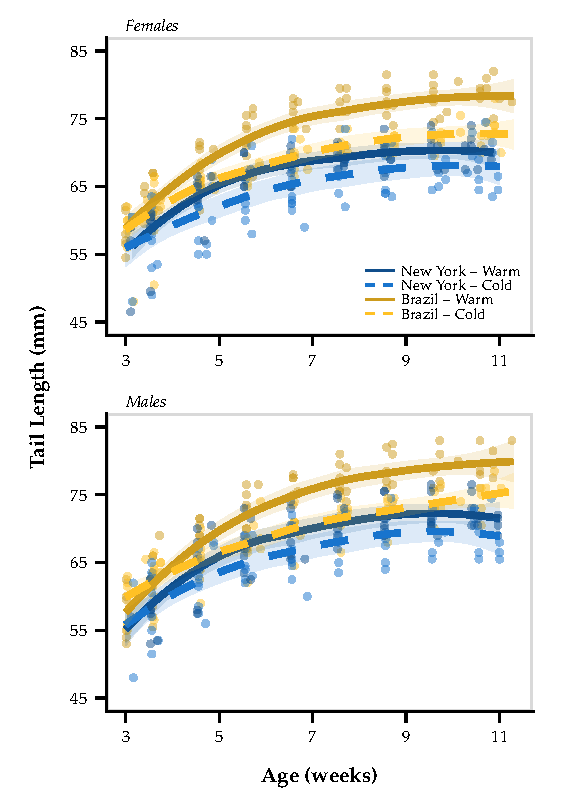
\includegraphics{../results/figures/Weekly_Tails.pdf}

\textbf{Figure 4. Tail length is highly influenced by cold temperature
across development.} Abslute tail length growth trajectories across
environments in New York (blue) and Brazil (gold) house mice.
Cold-reared mice (dotted lines) grow shorter tails compared to
warm-housed mice (solid lines). Both New York and Brazil house mice show
plasticity in response to temperature across tail development.
Individuals are plotted as semi-transparent points (n = 80), with
population means depicted as smoothed regression fits, with standard
error shading. The same individuals depicted here are also depicted in
Figure 6.

\newpage

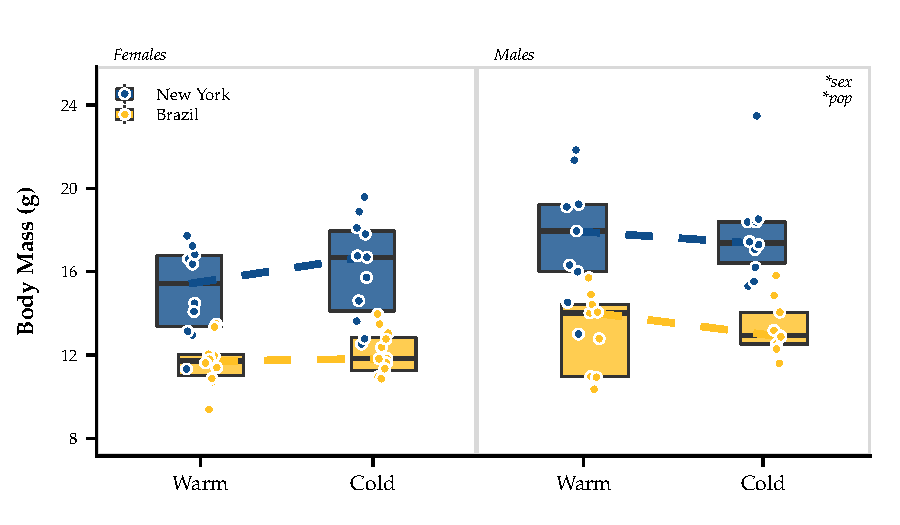
\includegraphics{../results/figures/RXNs_BW.pdf}

\textbf{Figure 5. Evolved variation and very little plasticity in body
size among New York and Brazil house mice.} Sexual dimorphism and strong
genetic components underlie body size differences among New York (blue)
and Brazil (gold) hosue mice. There is very little plasticity in body
mass in response to cold temperature. Individuals are represented as
individual points (n = 80). Boxplots denote the 25th, median, and 75th
quartiles. Results from linear mixed models are presented in each plot.
The same individuals depicted here are also depicted in Figure 3.

\newpage

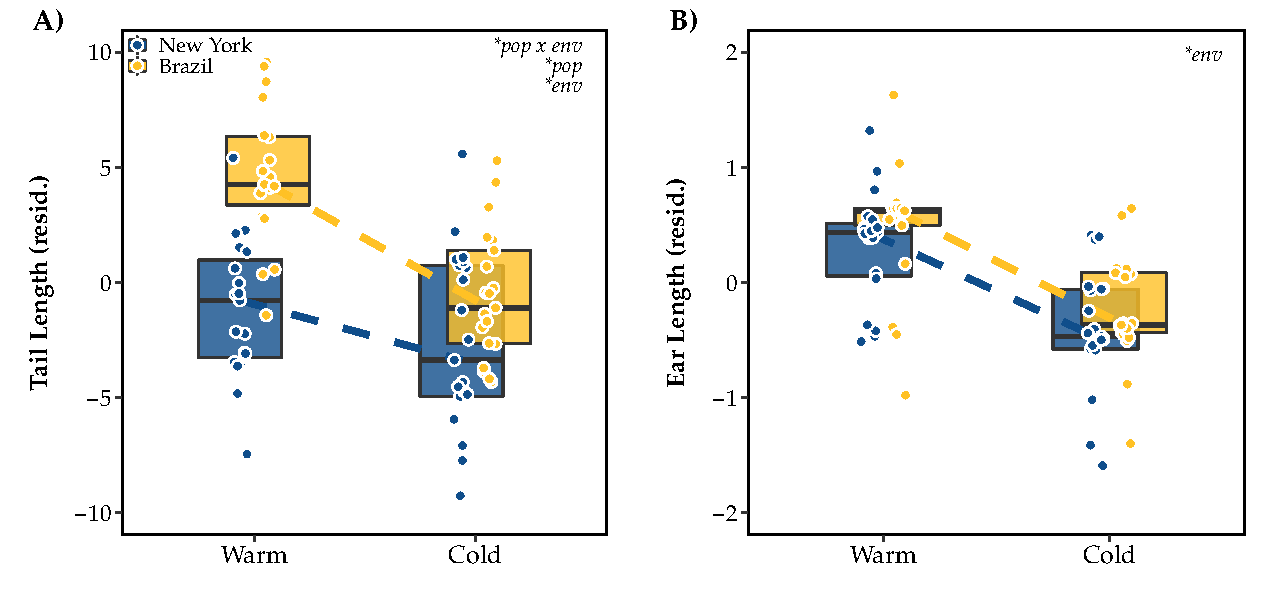
\includegraphics{../results/figures/RXNs_Extremities.pdf}

\textbf{Figure 6. Adaptive phenotypic plasticity in extremity length
among New York and Brazil house mice.} Evolved differences in tail
length among New York (blue) and Brazil (gold) house mice, with
warm-reared Brazil mice having longer tails than warm-reared New York
mice. Both tail length and ear length show significant plasticity in
both populations, with tails and ears growing shorter in the cold. The
plastic response of Brazil house mice goes in the same direction as the
evovled and plastic responses of New York house mice, highlighting an
example of adaptive plasticity in extremity length. Tail length and ear
length residuals were calculated by regressing from body mass.
Individuals are represented as individual points (tail length residuals:
n = 80; ear length residuals: n = 78). Boxplots denote the 25th, median,
and 75th quartiles. Both sexes were combined as there were no
sex-specific differences in extremity length. Results from linear mixed
models are presented in each plot. The same individuals depicted here
are also depicted in Figure 4.

\newpage

\hypertarget{acknowledgements}{%
\subsection{Acknowledgements}\label{acknowledgements}}

We are extremeley thankful to Kathleen Ferris, Gabriela Heyer, Dana Lin,
Felipe Martins, Megan Phifer-Rixey, Michael Sheehan, and Taichi Suzki
for collecting wild house mice, establishing wild-derived mouse
colonies, and maintaining colonies. M.A.B was supported by a National
Science Foundation Graduate Research Fellowship (DGE 1106400), Junea W.
Kelly MVZ Graduate Fellowship, and UC Berkeley Philomathia Graduate
Fellowship. This work was supported by an NIH grant to M.W.N.
(R01GM127468).

\newpage

\hypertarget{references}{%
\subsection{References}\label{references}}

\hypertarget{refs}{}
\leavevmode\hypertarget{ref-Alhajeri2020}{}%
Alhajeri, B. H., Y. Fourcade, N. S. Upham, and H. Alhaddad. 2020. A
global test of allen's rule in rodents. Global Ecology and Biogeography
29:2248--2260.

\leavevmode\hypertarget{ref-Alhajeri2016}{}%
Alhajeri, B. H., and S. J. Steppan. 2016. Association between climate
and body size in rodents: A phylogenetic test of bergmann's rule.
Mammalian Biology 81:219--225.

\leavevmode\hypertarget{ref-Allaire2021}{}%
Allaire, J., Y. Xie, J. McPherson, J. Luraschi, K. Ushey, A. Atkins, H.
Wickham, et al. 2021. Rmarkdown: Dynamic documents for r.

\leavevmode\hypertarget{ref-Allen1877}{}%
Allen, J. A. 1877. The influence of physical conditions in the genesis
of species. Radical Review 1:108--140.

\leavevmode\hypertarget{ref-Barnett1965}{}%
Barnett, S. 1965. Genotype and environment in tail length in mice.
Quarterly Journal of Experimental Physiology and Cognate Medical
Sciences: Translation and Integration 50:417--429.

\leavevmode\hypertarget{ref-Barnett1984}{}%
Barnett, S., and R. Dickson. 1984. Changes among wild house mice (mus
musculus) bred for ten generations in a cold environment, and their
evolutionary implications. Journal of Zoology 203:163--180.

\leavevmode\hypertarget{ref-Bates2015}{}%
Bates, D., M. Mächler, B. Bolker, and S. Walker. 2015. Fitting linear
mixed-effects models using lme4. Journal of Statistical Software
67:1--48.

\leavevmode\hypertarget{ref-Bergmann1847}{}%
Bergmann, C. 1847. Über die verhältnisse der wärmeökonomie der thiere zu
ihrer grösse. Gottinger Studien 3:595--708.

\leavevmode\hypertarget{ref-Betti2015}{}%
Betti, L., S. J. Lycett, N. von Cramon-Taubadel, and O. M. Pearson.
2015. Are human hands and feet affected by climate? A test of allen's
rule. American Journal of Physical Anthropology 158:132--140.

\leavevmode\hypertarget{ref-Blackburn2004}{}%
Blackburn, T. M., and B. A. Hawkins. 2004. Bergmann's rule and the
mammal fauna of northern north america. Ecography 27:715--724.

\leavevmode\hypertarget{ref-Brown1969}{}%
Brown, J. H., and A. K. Lee. 1969. Bergmann's rule and climatic
adaptation in woodrats (neotoma). Evolution 329--338.

\leavevmode\hypertarget{ref-Conover1995}{}%
Conover, D. O., and E. T. Schultz. 1995. Phenotypic similarity and the
evolutionary significance of countergradient variation. Trends in
Ecology \& Evolution 10:248--252.

\leavevmode\hypertarget{ref-Constable2010}{}%
Constable, H., R. Guralnick, J. Wieczorek, C. Spencer, A. T. Peterson,
V. S. Committee, and others. 2010. VertNet: A new model for biodiversity
data sharing. PLoS Biol 8:e1000309.

\leavevmode\hypertarget{ref-Endler1977}{}%
Endler, J. A. 1977. Geographic variation, speciation, and clines.
Princeton University Press.

\leavevmode\hypertarget{ref-Ferris2021}{}%
Ferris, K. G., A. S. Chavez, T. A. Suzuki, E. J. Beckman, M.
Phifer-Rixey, K. Bi, and M. W. Nachman. 2021. The genomics of rapid
climatic adaptation and parallel evolution in north american house mice.
PLoS genetics 17:e1009495.

\leavevmode\hypertarget{ref-Foster2013}{}%
Foster, F., and M. Collard. 2013. A reassessment of bergmann's rule in
modern humans. PloS one 8:e72269.

\leavevmode\hypertarget{ref-Fox2019}{}%
Fox, J., and S. Weisberg. 2019. An R companion to applied regression
(Third.). Sage, Thousand Oaks CA.

\leavevmode\hypertarget{ref-Freckleton2003}{}%
Freckleton, R. P., P. H. Harvey, and M. Pagel. 2003. Bergmann's rule and
body size in mammals. The American Naturalist 161:821--825.

\leavevmode\hypertarget{ref-Geist1987}{}%
Geist, V. 1987. Bergmann's rule is invalid. Canadian Journal of Zoology
65:1035--1038.

\leavevmode\hypertarget{ref-Gillespie1989}{}%
Gillespie, J. H., and M. Turelli. 1989. Genotype-environment
interactions and the maintenance of polygenic variation. Genetics
121:129--138.

\leavevmode\hypertarget{ref-Gomulkiewicz1992}{}%
Gomulkiewicz, R., and M. Kirkpatrick. 1992. Quantitative genetics and
the evolution of reaction norms. Evolution 46:390--411.

\leavevmode\hypertarget{ref-Griffing1974}{}%
Griffing, J. P. 1974. Body measurements of black-tailed jackrabbits of
southeastern new mexico with implications of allen's rule. Journal of
Mammalogy 55:674--678.

\leavevmode\hypertarget{ref-Husby2011}{}%
Husby, A., S. M. Hille, and M. E. Visser. 2011. Testing mechanisms of
bergmann's rule: Phenotypic decline but no genetic change in body size
in three passerine bird populations. The American Naturalist
178:202--213.

\leavevmode\hypertarget{ref-Huxley1938}{}%
Huxley, J. 1938. Clines: An auxiliary taxonomic principle. Nature
142:219--220.

\leavevmode\hypertarget{ref-James1970}{}%
James, F. C. 1970. Geographic size variation in birds and its
relationship to climate. Ecology 51:365--390.

\leavevmode\hypertarget{ref-James1983}{}%
---------. 1983. Environmental component of morphological
differentiation in birds. Science 221:184--186.

\leavevmode\hypertarget{ref-Johnston1971}{}%
Johnston, R. F., and R. K. Selander. 1971. Evolution in the house
sparrow. II. Adaptive differentiation in north american populations.
Evolution 1--28.

\leavevmode\hypertarget{ref-Kuznetsova2017}{}%
Kuznetsova, A., P. B. Brockhoff, and R. H. B. Christensen. 2017.
lmerTest package: Tests in linear mixed effects models. Journal of
Statistical Software 82:1--26.

\leavevmode\hypertarget{ref-Luxfcdecke2021}{}%
Lüdecke, D., M. S. Ben-Shachar, I. Patil, P. Waggoner, and D. Makowski.
2021. Assessment, testing and comparison of statistical models using r.
Journal of Open Source Software 6:3112.

\leavevmode\hypertarget{ref-Lynch1992}{}%
Lynch, C. B. 1992. Clinal variation in cold adaptation in mus
domesticus: Verification of predictions from laboratory populations. The
American Naturalist 139:1219--1236.

\leavevmode\hypertarget{ref-Mayr1956}{}%
Mayr, E. 1956. Geographical character gradients and climatic adaptation.
Evolution 10:105--108.

\leavevmode\hypertarget{ref-McNab1971}{}%
McNab, B. K. 1971. On the ecological significance of bergmann's rule.
Ecology 52:845--854.

\leavevmode\hypertarget{ref-Meiri2003}{}%
Meiri, S., and T. Dayan. 2003. On the validity of bergmann's rule.
Journal of biogeography 30:331--351.

\leavevmode\hypertarget{ref-Mincer2020}{}%
Mincer, S. T., and G. A. Russo. 2020. Substrate use drives the
macroevolution of mammalian tail length diversity. Proceedings of the
Royal Society B 287:20192885.

\leavevmode\hypertarget{ref-Nudds2007}{}%
Nudds, R., and S. Oswald. 2007. An interspecific test of allen's rule:
Evolutionary implications for endothermic species. Evolution:
International Journal of Organic Evolution 61:2839--2848.

\leavevmode\hypertarget{ref-Ozgul2010}{}%
Ozgul, A., D. Z. Childs, M. K. Oli, K. B. Armitage, D. T. Blumstein, L.
E. Olson, S. Tuljapurkar, et al. 2010. Coupled dynamics of body mass and
population growth in response to environmental change. Nature
466:482--485.

\leavevmode\hypertarget{ref-Ozgul2009}{}%
Ozgul, A., S. Tuljapurkar, T. G. Benton, J. M. Pemberton, T. H.
Clutton-Brock, and T. Coulson. 2009. The dynamics of phenotypic change
and the shrinking sheep of st. Kilda. Science 325:464--467.

\leavevmode\hypertarget{ref-Phifer-Rixey2018}{}%
Phifer-Rixey, M., K. Bi, K. G. Ferris, M. J. Sheehan, D. Lin, K. L.
Mack, S. M. Keeble, et al. 2018. The genomic basis of environmental
adaptation in house mice. PLoS Genetics 14:e1007672.

\leavevmode\hypertarget{ref-Ruff1994}{}%
Ruff, C. B. 1994. Morphological adaptation to climate in modern and
fossil hominids. American journal of physical anthropology 37:65--107.

\leavevmode\hypertarget{ref-Snow1954}{}%
Snow, D. 1954. Trends in geographical variation in palaerctic members of
the genus parus. Evolution 19--28.

\leavevmode\hypertarget{ref-Suzuki2020}{}%
Suzuki, T. A., F. M. Martins, Phifer-Rixey Megan, and M. W. Nachman.
2020. The gut microbiota and bergmann's rule in wild house mice.
Molecular Ecology 29:2300--2311.

\leavevmode\hypertarget{ref-Symonds2010}{}%
Symonds, M. R., and G. J. Tattersall. 2010. Geographical variation in
bill size across bird species provides evidence for allen's rule. The
American Naturalist 176:188--197.

\leavevmode\hypertarget{ref-Teplitsky2008}{}%
Teplitsky, C., J. A. Mills, J. S. Alho, J. W. Yarrall, and J. Merilä.
2008. Bergmann's rule and climate change revisited: Disentangling
environmental and genetic responses in a wild bird population.
Proceedings of the National Academy of Sciences 105:13492--13496.

\leavevmode\hypertarget{ref-Tomlinson2009}{}%
Tomlinson, S., and P. C. Withers. 2009. Biogeographical effects on body
mass of native australian and introduced mice, pseudomys
hermannsburgensis and mus domesticus: An inquiry into bergmann's rule.
Australian Journal of Zoology 56:423--430.

\leavevmode\hypertarget{ref-Via1985}{}%
Via, S., and R. Lande. 1985. Genotype-environment interaction and the
evolution of phenotypic plasticity. Evolution 39:505--522.

\leavevmode\hypertarget{ref-Wickham2019}{}%
Wickham, H., M. Averick, J. Bryan, W. Chang, L. D. McGowan, R. François,
G. Grolemund, et al. 2019. Welcome to the tidyverse. Journal of Open
Source Software 4:1686.

\leavevmode\hypertarget{ref-Yom-Tov1986}{}%
Yom-Tov, Y., and H. Nix. 1986. Climatological correlates for body size
of five species of australian mammals. Biological Journal of the Linnean
society 29:245--262.

\end{document}
